%%%%%%%%%%%%%%%%%%%%%%%%%%%%%%%%%%%%%%%%%%%%%%%%%%%%%%%%%%%%%%%%%%%%%%%%%
%%%%%%%%%%%%%%%%%%%%%%%%%      INTRODUÇÃO      %%%%%%%%%%%%%%%%%%%%%%%%%%
%%%%%%%%%%%%%%%%%%%%%%%%%%%%%%%%%%%%%%%%%%%%%%%%%%%%%%%%%%%%%%%%%%%%%%%%%

\section{\esp Introdução} \label{intro}

Instituída em 10 de dezembro de 2009, a Lei n.º 12.116/2009 \citeonline{lei}, conforme o Congresso Nacional Brasileiro, decreta o dia 27 de novembro como o Dia Nacional de Luta contra o Câncer de Mama. Além de uma data específica para a luta contra esse câncer, foi criada em 1990, uma campanha cujo objetivo é conscientizar a população sobre a importância da prevenção e do diagnóstico precoce, o chamado Outubro Rosa.

Causado pela multiplicação rápida e desordenada de células anormais, o câncer pode ocorrer em diversas estruturas do corpo, e quando envolve as células das glândulas mamárias, determina o câncer de mama \cite{incaoquee}. Esse tumor divide a primeira posição com o de pulmão no ranking dos cânceres mais incidentes do mundo, além de ser a doença mais comum entre as mulheres, na qual dados da Organização Mundial de Saúde (OMS) e do Instituto Nacional de Câncer (INCA) apontam que ocorrem por volta de 627 mil mortes por câncer de mama no mundo em 2018, sendo 17,7 mil no Brasil \cite{boletimepidemiologico}.

O diagnóstico prévio dessa doença tem alta significância na contenção do progresso da doença, devido à introdução antecipada do tratamento, que favorece o crescimento das chances de sobrevivência do paciente diagnosticado. Diante disso, existem alguns procedimentos basilares empregados para o diagnóstico dessa doença, tais quais: o exame de toque; exames clínicos; exames de imagens como a mamografia, ultrassonografia ou ressonância magnética; e a confirmação via biópsia.

% Problema Escolhido: já está incluso nesse parágrafo.
De acordo com \citeonline{borchartt}, a mamografia é o exame mais comum para a detecção do câncer de mama, mas apresenta algumas limitações, especialmente para mulheres mais jovens e com o tecido mamário denso. Perante o avanço computacional, a termografia se destaca como uma técnica de diagnóstico não invasiva que permite interceptar diferenças de temperatura em diferentes regiões do corpo através da intensidade da radiação infravermelha. Quando aplicada ao câncer de mama, a termografia se torna uma ferramenta essencial para a detecção prévia da doença. Isso porque as células cancerígenas tendem a apresentar temperaturas mais elevadas do que as células normais, independentemente de fatores como idade e outros \cite{leles}.

% Motivações
Com a evolução da computação em diversos âmbitos tecnológicos, tais como redes neurais, processamento de imagens e inteligências artificiais, oportunidades foram criadas para investigar e implementar soluções avançadas na área da saúde, visando agregar a comunidade médica, além da sociedade no geral. Na oncologia, existem diversos métodos e práticas utilizadas para diagnosticar um quadro de câncer de um paciente, porém, em sua grande maioria, requer uma análise humana que é passiva de erros ou até mesmo incapaz de realizar predições, ou quantificar com precisão o diagnóstico do quadro clínico \cite{parametrization}.

Pautando-se na ideia de trazer ferramentas que auxiliam médicos no diagnóstico antecipado do câncer de mama, algoritmos de processamento de imagem e predição podem melhorar a tomada de decisões dos profissionais de saúde acerca do quadro geral dos pacientes. Dessa maneira, o tratamento pode ser iniciado previamente, podendo evitar a progressão do câncer para estágios mais avançados, que são mais difíceis de tratar, e aumentando as chances de cura, reduzindo a necessidade de tratamentos invasivos. À vista disso, os equipamentos desenvolvidos com esse propósito garantem uma qualidade de vida e longevidade maior para todos assolados pelo quadro de câncer.

% Objetivos
Diante do contexto levantado, o presente artigo apresenta uma metodologia para a identificação de células cancerosas, que utiliza o processamento e análise de imagens termográficas por meio de Aprendizado por Transferência (do inglês \textit{Transfer Learning}). Outrossim, para investigar de maneira experimental o tema proposto neste artigo, foram utilizadas bases de dados, criteriosamente selecionadas e normalizadas em termos de tamanho e histograma, contendo amostras de mamografias para o treinamento de um algoritmo de inteligência artificial desenvolvido. As amostras foram divididas em mamografias sem sinais de câncer e mamografias com câncer, classificadas de acordo com seus respectivos graus. Todos os códigos desenvolvidos e as bases de dados utilizadas estão disponíveis publicamente no \textit{GitHub}\footnote{\href{https://github.com/Vaftir/TCC_master/}{\textit{https://github.com/Vaftir/TCC\_master/}}}.

Para criar um modelo de classificação de graus, foi utilizado o método de \textit{Deep Learning}, que consiste em uma técnica avançada de Aprendizado de Máquina (do inglês \textit{Machine Learning}). Após o treinamento do modelo, sua acurácia foi avaliada por meio de testes, e assim que devidamente treinado, o algoritmo foi capaz de analisar as imagens dos exames mamográficos e realizar uma classificação precisa e automatizada do câncer de mama, identificando o grau da doença, caso presente no paciente.

O restante deste artigo está estruturado da seguinte maneira: a seção \ref{fundteorica} apresenta o referencial teórico, na seção \ref{trabcorr} é fornecida uma visão geral dos trabalhos correlatos encontrados na literatura, a seção \ref{metodologia} descreve a metodologia, dividida em materiais e métodos, e, por fim, a seção \ref{results} apresenta os resultados preliminares. 


%%%%%%%%%%%%%%%%%%%%%%%%%%%%%%%%%%%%%%%%%%%%%%%%%%%%%%%%%%%%%%%%%%%%%%%%%
%%%%%%%%%%%%%%%%%%%      FUNDAMENTAÇÃO TEÓRICA       %%%%%%%%%%%%%%%%%%%%
%%%%%%%%%%%%%%%%%%%%%%%%%%%%%%%%%%%%%%%%%%%%%%%%%%%%%%%%%%%%%%%%%%%%%%%%%


\section{\esp Fundamentação teórica}  \label{fundteorica}

De modo a fornecer informações mais detalhadas sobre os tópicos vitais para a compreensão do presente artigo, esta seção retrata conceitos fundamentais sobre o câncer de mama, exames e tratamentos para a doença, bem como técnicas de processamento de imagens termográficas. Além disso, será discutida a técnica de \textit{Deep Learning} com o uso de imagens para demonstrar sua relevância no contexto da detecção do câncer de mama.

%%%%%%%%%%%%%%%%%%%%%%      CÂNCER DE MAMA       %%%%%%%%%%%%%%%%%%%%%%%

\subsection{\esp Câncer de mama} \label{cancerdemama}
As células vivas que compõem o corpo humano se dividem para permitir o crescimento e a substituição de células danificadas ou mortas. A proliferação celular é regulada pelos genes do Ácido Desoxirribonucleico (DNA, do inglês Deoxyribonucleic Acid), transmitidos pelos pais e gerenciados para manter o equilíbrio no processo de divisão celular. O câncer, em geral, se forma quando esse controle genético é danificado ou perdido em uma, ou mais células que então continuam a se dividir normalmente, produzindo mais células anormais, causando danos a outros tecidos e funções corporais \cite{basicOncology}.

O câncer de mama, em específico, se dá pelo crescimento de células anormais na glândula mamária, e os sub-tipos diferentes desse câncer estão localizados sob o tecido adiposo (tecido que armazena gordura e mantém a maior reserva de energia do organismo) e no sistema ductal (ductos responsáveis por conduzir o leite até a papila). Conforme apontado por \citeonline{souza}, o câncer de mama apresenta células com uma taxa de duplicação de tamanho estimada em 4 meses. Embora o crescimento seja inicialmente lento, quando o tumor se torna palpável e não é tratado, o câncer pode se disseminar para os linfonodos, pulmões, ossos, fígado e cérebro, desenvolvendo metástase.

A descoberta prévia do câncer de mama aumenta significativamente a probabilidade de um paciente se curar da doença, dependendo de qual método for utilizado para a detecção. Com isso, é necessário avaliar se o método escolhido é invasivo ou não. No passado, os equipamentos de medição de emissão infravermelha eram capazes de captar uma variação de temperatura apenas de 0,5 a 1 °C, utilizando uma tecnologia primitiva que exigia que um filme de cristal líquido fosse colocado nos seios dos pacientes para detectar a temperatura. Ainda assim, segundo \citeonline{noninvasive}, as câmeras de termografia infravermelhas digitais conseguem identificar mudanças de 0,08 °C, em adição de não demandar contato físico com o paciente.


%%%%%%%%%%%%%%%%%%%%%%     PROCESSAMENTO DE IMAGEM       %%%%%%%%%%%%%%%%%%%

\subsection{\esp Processamento de Imagem} \label{procesamentoimg}

Matematicamente, uma imagem pode ser descrita como uma função bidimensional, f(x, y), onde x e y representam coordenadas espaciais, e a amplitude de f em qualquer par de coordenadas é chamada de a intensidade ou nível de cinza da imagem naquele ponto \cite{techniques}. Quando x, y e os valores de intensidade de f são quantidades finitas e discretas, chamamos a imagem de imagem digital. É essencial que uma imagem digital seja composta por um número finito de elementos (conhecidos como \textit{pixels}, \textit{pels} ou elementos de imagem), cada um com sua própria localização e valores específicos. 

A definição básica de processamento de imagem refere-se ao processo de tratamento de imagens digitais, incluindo a remoção de ruídos e outros tipos de irregularidades presentes \cite{histopathological}. Durante as últimas quatro a cinco décadas, várias técnicas foram desenvolvidas no campo de processamento de imagens, sendo a maioria desenvolvida para aprimorar imagens obtidas por espaçonaves não tripuladas, sondas espaciais e aeronaves militares de reconhecimento. Devido a fácil disponibilidade de computadores poderosos, dispositivos de memória de grande porte e software gráfico, os sistemas de processamentos de imagem estão se tornando cada vez mais populares. Uma das principais vantagens dos métodos de processamento é versatilidade, repetibilidade e preservação da precisão dos dados originais, utilizando técnicas como: i) Pré-processamento, ii) Melhoria, iii) Segmentação, iv) Extração de recursos, e v) Classificação \cite{lungcancer}.

As imagens capturadas por satélites e câmeras convencionais ou digitais carecem de contraste e brilho devido a limitações nos subsistemas de imagem, ou condições de iluminação durante a captura. Além disso, segundo \citeonline{techniques}, essas imagens podem conter diferentes tipos de ruído. Nesse contexto, o aprimoramento de imagem procura acentuar certas características da imagem para análise posterior ou exibição. Os exemplos incluem contraste e retoque de borda, pseudo-coloração, filtragem de ruído, nitidez e ampliação. As técnicas de aperfeiçoamento, que englobam alargamento de contraste, conforme mostrado na Figura \ref{fig:contraste}, modificação do histograma e filtragem de ruído, consoante à Figura \ref{fig:ruido}, são úteis na extração de recursos, análise e exibição. Entretanto, o próprio processo de aprimoramento não aumenta o conteúdo de informações inerentes aos dados, enfatizando somente certas características de imagem especificadas. Algoritmos de aprimoramento são geralmente interativos e dependentes de aplicativos.

 \begin{figure}[ht]
 	\centering	
 	\caption[\hspace{0.1cm}Grade Computacional.]{Alargamento de Contraste}
 	\vspace{-0.4cm}
 	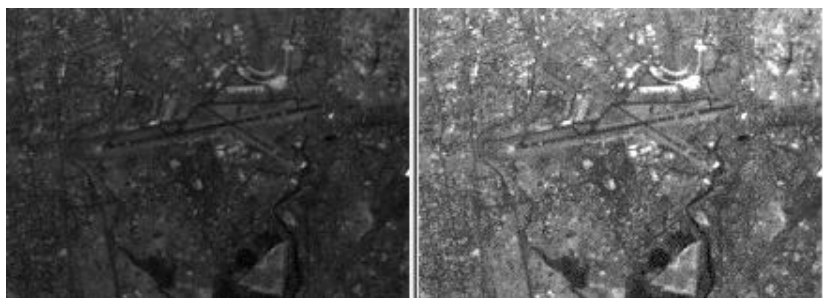
\includegraphics[width=0.5\textwidth]{figuras/Alargamento de Contraste.png}
 	\captionsetup{justification=centering}
	\vspace{-0.2cm}
	\\\textbf{\footnotesize Fonte: \cite{techniques} }
	\label{fig:contraste}
\end{figure}

 \begin{figure}[ht]
 	\centering	
 	\caption[\hspace{0.1cm}Grade Computacional.]{Retirada de Ruido}
 	\vspace{-0.4cm}
 	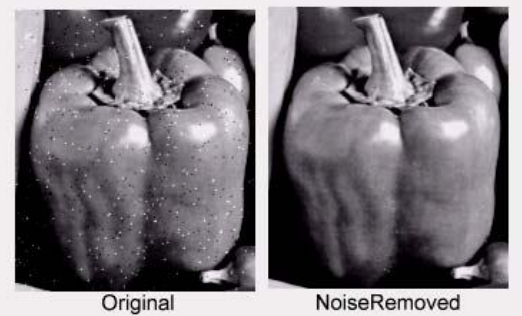
\includegraphics[width=0.5\textwidth]{figuras/Retirada de Ruido.png}
 	\captionsetup{justification=centering}
	\vspace{-0.1cm}
	\\\textbf{\footnotesize Fonte: \cite{techniques} }
	\label{fig:ruido}
\end{figure}



%%%%%%%%%%%%%%%%%%%%%%%%%%     DEEP LEARNING       %%%%%%%%%%%%%%%%%%%%%%

\subsection{\esp Deep Learning} \label{deeplearning}

O Machine Learning é um processo que utiliza uma gama de dados para criar uma inteligência artificial instruído para aprender e operar funções de maneira autônoma \cite{machinelearning}. Dentre as abundantes formas de se aplicar esse processo, uma das mais comuns é o método \textit{Deep Learning}, que utiliza redes neurais convolucionais para criar aplicações mais completas. 


O termo \textit{Deep Learning} refere-se à estrutura utilizada para realização do método, que consiste em várias camadas de neurônios artificiais conectados, permitindo que o sistema aprenda representações cada vez mais complexas dos dados de entrada. Esses dados podem variar desde um simples conjunto de inteiros, para fazer uma predição de cálculo, até um sistema de navegação de um veículo autônomo \cite{deeplearning}.

Os neurônios artificiais são a principal composição da rede neural, sendo estruturas agrupadas em camadas, inspiradas nos neurônios biológicos presentes no cérebro humano. Cada neurônio artificial recebe diversas entradas, representadas por valores numéricos, multiplicadas por um determinado peso e somados. Esse resultado é então processado mediante uma função de ativação, que determina a saída do neurônio, e é transmitida para os outros neurônios da rede.



%%%%%%%%%%%%%%%%%%%%%%%%%%     REDES NEURAIS       %%%%%%%%%%%%%%%%%%%%%%

\subsection{\esp Redes Neurais} \label{redesneurais}

A Rede Neural Convolucional  (CNN, do inglês \textit{Convolutional Neural Network}), de acordo com \citeonline{cnn}, é uma estrutura complexa composta por inúmeros neurônios e camadas de convolução compostas por um conjunto de filtros que, por sua vez, detectam características visuais específicas em uma imagem por meio de uma matriz. Sua arquitetura pode ser dividida em três camadas individuais: i) Camada de Entrada (do inglês \textit{Input Layer}), ii) Camadas Escondidas (do inglês \textit{Hidden Layers}), e iii) Camada de Saída (do inglês \textit{Output Layer}), com funções de entrada, processamento, e saída de dados respectivamente \cite{medical}.

Na camada de entrada, os dados brutos, como fotos e vídeos, são recebidos e transformados em dados matemáticos enviados para as camadas seguintes da CNN \cite{cnn}. Nas camadas escondidas, são usadas funções matemáticas não-lineares modeladas para retornar valores específicos, consoantes os dados de entrada. Esses valores são então enviados para a última parte da rede. Por fim, na camada de saída, é produzido o resultado com base nas predições das camadas anteriores.





%%%%%%%%%%%%%%%%%%%%%%%%%%%%%%%%%%%%%%%%%%%%%%%%%%%%%%%%%%%%%%%%%%%%%%%%%
%%%%%%%%%%%%%%%%%%%%      TRABALHOS CORRELATOS       %%%%%%%%%%%%%%%%%%%%
%%%%%%%%%%%%%%%%%%%%%%%%%%%%%%%%%%%%%%%%%%%%%%%%%%%%%%%%%%%%%%%%%%%%%%%%%


\section{\esp Trabalhos correlatos} \label{trabcorr}

Nesta seção, são abordados trabalhos correlatos que utilizam inteligência artificial para o diagnóstico de câncer, se diferenciando em termos de entrada de imagem (como radiografias ou imagens digitais), além de apresentar as bases de dados usadas, abordagens, algoritmos e análises dos resultados. 

Em \citeonline{marinePredators}, é proposto um modelo de detecção de câncer de mama. O trabalho alcançou uma acurácia de 92\%, normalizando as imagens termográficas e utilizando o \textit{Marine-Predators-Algorithm} que auxilia na otimização da seleção das características (definidas por algumas técnicas de reconhecimento de padrões) mais relevantes das imagens e parâmetros do modelo de observação. Para classificar e validar a implementação feita, foram utilizadas variantes (tipos de funções matemáticas que medem a similaridade entre dois pontos no espaço) do algoritmo de Máquina de Vetores de Suporte (SVM, do inglês \textit{Support Vector Machine}).

Por outro lado, \citeonline{comparing} ao utilizar outra abordagem de treinamento do algoritmo, chegou em 61,8\% de precisão dos resultados. Foi utilizado o método de limiarização por refinamento adaptativo, técnica que segmenta uma imagem em duas ou mais (com base nos valores dos \textit{pixels}), de modo que regiões anormais são identificadas com mais precisão. Além disso, o artigo também compara o resultado entre suas métricas com outros trabalhos, e com base nisso, concluiu-se que a inconsistência das comparações foi devido ao uso de imagens infravermelhas distintas, uma vez que foram utilizadas 102 imagens de uma base de dados pública.
%Diz q usa limiarização baseado na Section III .ASPECTS OF THE APPLIED APPROACH: "In our approach we have used the same methodology that composed the automatic ROI segmentation developed in [19] that was proven to produce good results regarding a comparison to a (...)"

Assim como o trabalho anterior, \citeonline{segmentacao} utiliza da limiarização por refinamento adaptativo, todavia, com uma acurácia de 96\%. Foram introduzidos três parâmetros para avaliação, baseando-se na informação de que as pregas mamárias (área indicadora de limites inferiores da mama, pois possuem maior temperatura) podem variar de tamanho, dificultando a identificação das mamas. Os parâmetros determinam miliares mínimos de uma área medida em \textit{pixels} que a prega deve ter, além de definir a área mínima a ser medida em \textit{pixel} para duas componentes distintas. Com isso, foi possível determinar qual conjunto de parâmetros maximiza as métricas estatísticas apresentadas, determinando assim os resultados normalizados.

Como aplicado em \citeonline{MachineVision}, foram desenvolvidas técnicas de Visão de Máquina (do inglês \textit{Machine Vision}), algoritmo que processa imagens e reconhece características básicas, em contrapartida à técnicas de processamento de imagens, em que a saída é outra imagem, entretanto, devidamente tratada. Com o uso de linguagens de alto nível confiáveis e eficientes, inúmeros algoritmos foram otimizados resultando na criação de poderosas ferramentas acessíveis para pesquisadores e cientistas, aumentando a precisão dos resultados. A discussão da Visão de Máquina básica e algoritmos de processamento de imagem do artigo foram implementados em cinco grupos principais: 
\begin{enumerate}
  \renewcommand{\labelenumi}{\alph{enumi})}
    \item Técnicas de Segmentação ou Limiar em \textit{Grey-Level}: utilizando métodos como \textit{P-tile} (histogramas), \textit{Edge Pixel} e \textit{Interative};
    
    \item Técnicas de Detecção de Borda: localização da borda para aumentar o contraste, utilizando o algoritmo \textit{Canny Edge Detection};
    
    \item Morfologia Digital: filtra a imagem, além de fazer uma análise geométrica da estrutura dos elementos;
    
    \item Textura: observação da repetição de padrões a fim de substitui-los usando \textit{grey level};
    
    \item Algoritmos de Esqueletização e Encurtamento: definir propriedades globais dos objetos e reduzir a imagem em um modelo mais compacto para reconhecer padrões.
\end{enumerate}


Utilizando redes neurais para reconhecer imagens de câncer de pele e unindo técnicas de processamento de imagens digitais, \citeonline{botelho} possibilita a elaboração de um sistema que diferencia imagens de Melanomas. Para isso, quatro características são usadas para identificar uma lesão: assimetria, bordas irregulares, cor variada e diâmetro. Baseados nessas características, o modelo proposto implementa a rede neural \textit{Perceptron} de Camada Única, utilizando dois neurônios: um excitado por imagens de lesões Melanoma, e outro excitado por imagens de lesões não Melanoma. O \textit{Perceptron} identifica quando uma entrada é classificada erroneamente e ajusta os pesos por meio de uma regra de correção de erro, conhecida como Regra Delta. Com isso, a rede é treinada somente quando todas as saídas correspondem com a saída esperada, atingindo uma taxa de 69\% de acertos.

\citeonline{NakagamiImages} apresenta uma abordagem baseada em \textit{Deep Learning} para detecção e classificação de massas na mama combinando imagens de ultrassom \textit{B-mode} e Nakagami, para fornecer informações complementares sobre o padrão de dispersão de tecidos. O ultrassom B-mode consiste em uma técnica que utiliza ondas sonoras de alta frequência enviadas ao corpo, e refletidas pelos tecidos internos, criando uma imagem em escala cinza aonde as áreas mais brilhantes representam tecidos mais densos. Já as imagens Nakagami são geradas a partir da análise das amplitudes de sinal retornadas pelo tecido examinado, fornecendo informações sobre a presença de diferentes tipos de estruturas. Utilizando uma arquitetura de rede neural convolucional para extrair características das imagens combinadas, as massas são classificadas como malignas ou benignas. Por fim, a abordagem proposta foi provada altamente eficaz na localização de massas, com uma precisão de 91,8\%, um desempenho significativamente melhor do que as abordagens existentes que usam apenas imagens B-mode ou Nakagami.

Em \citeonline{systematic}, os autores analisaram os diferentes tipos de Redes Neurais Artificiais (ANN, do inglês \textit{Artificial Neural Network}) e modelos de \textit{Deep Learning} já utilizados na literatura para processar imagens termográficas de câncer de mama. Mesmo que a termografia, seja atualmente o melhor método para a descoberta precoce, a qualidade das imagens é um desafio tangível. O processo de melhoramento da imagem tenta mostrar detalhes escondidos e destacar características para que a profundidade e tamanho do tumor sejam distinguidos de um tecido saudável. Para melhorar a qualidade da imagem, o trabalho utiliza um dispositivo de resfriamento de mama. Além disso, são destacadas as contribuições e desvantagens de trabalhos relacionados que empregam termografia e inteligência artificial, obtidos mediantes comparações feitas no decorrer do artigo e são desenvolvidos questionamentos a cerca dos desafios enfrentados, como a falta de padronização na aquisição de imagens térmicas e a necessidade de mais dados de treinamento para as redes neurais. 

Para desenvolver uma técnica precisa e eficiente para a identificação antecipada do câncer de mama, \citeonline{ChaoticSalp} usaram a segmentação de imagens térmicas em conjunto com o algoritmo \textit{Chaotic Salp Swarm}. O algoritmo proposto consiste em uma técnica de otimização bioinspirada, usada para ajustar os parâmetros de segmentação das termografias e encontrar as regiões suspeitas de câncer de mama. Assim como o anterior, foi utilizada uma base de dados pública de imagens térmicas para avaliar a eficácia do método proposto. Os resultados obtidos foram avaliados baseados em métricas como: sensibilidade, especificidade e coeficiente de Dice. Não é especificado o índice de precisão do trabalho, entretanto, é considerado que o método proposto teve um desempenho satisfatório em termos de precisão na segmentação de regiões suspeitas de câncer de mama nas imagens térmicas.

\citeonline{borchartt} teve como foco a análise das potenciais contribuições que o uso de imagens infravermelhas tem para diagnósticos de doenças na mama. Para o estudo, foram utilizadas 102 imagens Infravermelhas (IR, do inglês \textit{Infrared Radiation}) de mama única da base de dados público da Pro Engenharia (PROENG) (sendo 47\% com alguma anormalidade) e resultados foram obtidos através do uso de algoritmos para detecção de condições malignas, como SVM, para extrair as características como primeiro momento, terceiro momento, não uniformidade da massa cinzenta e porcentagem de execução. Os autores expõem a dificuldade em realizar o processo de segmentação da região da mama, extração da região de interesse, devido à natureza amorfa e a falta de limites claros. Além disso, é apontado que ao usar uma base de dados público para comparar as imagens e extrair características, os melhores resultados foram obtidos com o classificador \textit{Sequential Minimum Optimization} (SMO), em adição a expor a inconsistência da comparação entre trabalhos que utilizam imagens IR. 

Buscando explorar métodos não invasivos para a localização precoce do câncer de mama, \citeonline{leles} propõe o uso de imagens térmicas que permitem detectar mudanças na temperatura, causadas pelo aumento do fluxo sanguíneo na área afetada pelo tumor. Após o pré-processamento, foi feito o refinamento manual da região de interesse para que alguns atributos extraídos não colaborassem com dados de fora da mama. Avaliando 70 pacientes, o trabalho identifica a temperatura máxima, mínima e média das mamas para utilizar no cálculo da sensibilidade (capacidade do teste em identificar corretamente o diagnóstico) e especificidade (capacidade do teste em excluir corretamente os que não tem a doença), com os valores de 92,3\% e 86,2\%, respectivamente.

A fim de abordar a detecção de metástase em linfonodos axilares em pacientes com câncer de mama, \citeonline{ashokkumar} utiliza o método de \textit{Data Augmentation} que faz modificações geométricas das imagens (como rotação, inversão, deslocamento e dimensionamento). Isso fornece uma garantia de que o modelo se concentra em áreas de câncer de mama, em vez de fontes de ruído aleatórias. Conforme o texto, foi demonstrado que o método ajuda na memorização de qualidades específicas das imagens treinadas, e evita que as redes se tornem superajustadas, ou seja, um modelo de aprendizado profundo que se adaptou demasiadamente nos dados de treinamento a ponto de não conseguir capturar padrões mais amplos. Além disso, usando ANN, o trabalho alcançou 98\% de acurácia superando modelos de radiografia.


%%%%%%%%%%%%%%%%%%%%%%%%%%%%%%%%%%%%%%%%%%%%%%%%%%%%%%%%%%%%%%%%%%%%%%%%%
%%%%%%%%%%%%%%%%%%%%%%%%      METODOLOGIA       %%%%%%%%%%%%%%%%%%%%%%%%%
%%%%%%%%%%%%%%%%%%%%%%%%%%%%%%%%%%%%%%%%%%%%%%%%%%%%%%%%%%%%%%%%%%%%%%%%%


\section{\esp Metodologia} \label{metodologia}
A fim de aprofundar os fundamentos do tema abordado, esta seção apresenta os recursos e ferramentas utilizados para a implementação do algoritmo, bem como informações técnicas relacionadas a linguagens de programação, bibliotecas e base de dados.


%%%%%%%%%%%%%%%%%%%%%%%     MATERIAIS       %%%%%%%%%%%%%%%%%%%%%%

\subsection{\esp Materiais} \label{materiais}


%%%%%%%%%%%%%%%%%%%%%%%     BASE DE DADOS       %%%%%%%%%%%%%%%%%%%%%%
\subsubsection{\esp Base de Dados} \label{database}

As amostras de imagens termográficas foram obtidas por meio do projeto PROENG \citeonline{database}, cujo objetivo é auxiliar no diagnóstico por meio de imagens médicas. O projeto abrange desde a aquisição das imagens até sua organização na base de dados bem como análises e técnicas de \textit{Machine Learning}. O \textit{Visual Lab DMR}\footnote{\href{http://visual.ic.uff.br/dmi}{\textit{http://visual.ic.uff.br/dmi}}} (Banco de Dados para Pesquisas em Mastologia, do inglês \textit{Database for Mastology Research}) é uma plataforma online que armazena imagens termográficas e mamografias, permitindo também que indivíduos voluntários contribuam inserindo suas próprias imagens, com o intuito de auxiliar em pesquisas na área da mastologia.

O conjunto de dados coletados no \textit{Visual Lab DMR}, consiste em imagens de 83 pacientes com câncer e imagens de 142 pacientes sem câncer, totalizando 225 pacientes. Cada paciente possui, em média, 25 imagens capturadas em diferentes posições, incluindo frontal, lateral direita, lateral esquerda e outros ângulos.


%%%%%%%%%%%%%%%%%%%%%%%     TECNOLOGIAS       %%%%%%%%%%%%%%%%%%%%%%

\subsubsection{\esp Tecnologias} \label{techs}
Para desenvolver o algoritmo de classificação das imagens entre pacientes com câncer e pacientes sem câncer, foram empregadas diversas tecnologias e bibliotecas, em conjunto com uma linguagem de programação, visando facilitar o processo. Para reproduzir a implementação, foi necessário configurar o sistema operacional do computador com o \textit{Python}, uma linguagem de programação de alto nível, interpretada, com tipagem dinâmica, além de incluir orientação a objetos, diversas bibliotecas e suporte a módulos e pacotes. A implementação requer o \textit{Python} com uma versão entre 3.7 e 3.10.


Adicionalmente, para gerenciar as dependências do projeto, foi utilizado um gerenciador de pacotes para o \textit{Python} (por exemplo, utilizando o comando "\textit{pip install <pacote>}", onde <pacote> representa o nome do pacote a ser instalado). Algumas das principais bibliotecas utilizadas são:

\begin{enumerate}[label=\alph*)]
    \item \textit{TensorFlow}: desenvolve modelos de \textit{Machine Learning}.
    
    \item \textit{Keras}: usada em conjunto com o \textit{TensorFlow}, permitindo construção e treinamento de redes neurais.
    
    \item \textit{PIL}: oferece recursos para o processamento de imagens, como abrir, manipular e salvar em diferentes formatos.
        
    \item \textit{matplotlib}: para visualização de dados, permitindo criar gráficos, \textit{plots}, histogramas, entre outros.
    
    \item \textit{numpy}: aplicada para computação e análise numérica, fornecendo uma estrutura de dados como vetores multidimensionais para armazenar grandes conjuntos de dados numéricos.

    \item \textit{os}: interage com o sistema operacional, permitindo manipulação de diretórios, entre outros.

    \item \textit{cv2}: fornece funções para carregar, manipular e processar imagens.

    \item \textit{time}: medição de tempo e manipulação de datas.

    \item \textit{glob}: realiza operações de pesquisa de arquivos e diretórios.

    \item \textit{random}: gera números aleatórios e funções de aleatoriedades.
\end{enumerate}


%%%%%%%%%%%%%%%%%%%%%%%     MÉTODOS       %%%%%%%%%%%%%%%%%%%%%%


\subsection{\esp Métodos} \label{metodos}

Nesta seção, são apresentadas as metodologias para o treinamento de um modelo de rede neural convolucional fazendo uso de bibliotecas do \textit{Python}. O método proposto consiste em cinco etapas: base de imagens, pré-processamento, aplicação do método de \textit{Transfer Learning}, declaração do modelo e predições. O código-fonte e a base de dados do projeto podem ser encontrados em um repositório hospedado no \textit{Github}.

%TODO: !!!!!!!!!!!!!!!!!!!!!!!!!!!!!!!!!!!!!!!!!!!!!!!!!!!!!!!!!!!!!!!!!!!!!!!!!!!!!!!!!!!!!!!!!!!!!!!!!!!!!!!!!!!!!!!!!!!DIAGRAMA!!!!!!!!!!!!!!!!!!!!!!!!!!!!!!!!!!!!!!!!!!!!!!!!!!!!!!!!!!!!!!!!!!!!!!!!!!!!!!!!!!!!!!!!!!!!!!!!!!!!!!!!!!!!!!!!!!!


%%%%%%%%%%%%%%%%%%%%%%%     PRÉ-PROCESSAMENTO       %%%%%%%%%%%%%%%%%%%%%%

\subsubsection{\esp Pré-Processamento} \label{preprocess}
Inicialmente é necessário importar as bibliotecas necessárias, conforme descrito na seção \ref{techs}, para o desenvolvimento do código. Estas fornecem funcionalidades e recursos necessários para a implementação do algoritmo. Ademais, foram carregadas 4530 imagens como dados de treinamento e 4530 imagens como dados de validação do modelo.

Em seguida, o pré-processamento das imagens é feito, gerando assim o vetor para o treinamento. Essa etapa foi realizada a partir da utilização da biblioteca \textit{ImageDataGenerator}. Originada do \textit{TensorFlow}, essa biblioteca permite transformar as imagens em dados vetoriais, facilitando os cálculos necessários durante o treinamento do modelo. Definimos uma instância do \textit{ImageDataGenerator}, que servirá para aplicar os métodos de transformação em vetor. Dentro desse método, existe um parâmetro chamado \textit{rescale} utilizado para fazer a normalização dos valores dos \textit{pixels} das imagens, transformando os valores originais dos \textit{pixels} em uma escala específica. Essa escala, geralmente, é utilizada com o valor de 1/255, uma vez que as imagens utilizadas na implementação consistem em coeficientes Vermelho, Verde, Azul (RGB, do inglês \textit{Red, Green, Blue}), ou seja, cada \textit{pixel} tem um valor entre 0 e 255. Entretanto, esses valores são grandes demais para o modelo proposto processar, conforme a taxa de aprendizado comum. Por conta disso, os valores foram realinhados para se distinguir entre 0 e 1.

%  \begin{figure}[ht]
%  	\centering	
%  	\caption[\hspace{0.1cm}Grade Computacional.]{Instância da biblioteca \textit{ImageDataGenerator} e Pré-Processamento}
%  	\vspace{-0.4cm}
%  	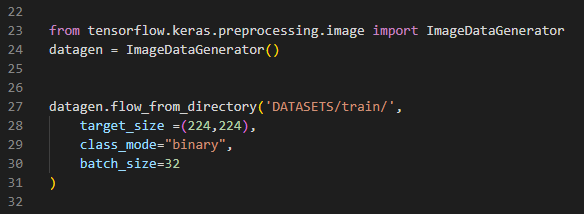
\includegraphics[width=1\textwidth]{figuras/imggenerator.png}
%  	\captionsetup{justification=centering}
%      \\\textbf{\footnotesize Fonte: \textit{GitHub}}
% 	\label{fig:generator}
% \end{figure}


Além disso, utilizamos o método \textit{flow\_from\_directory} para pré-processar os dados que serão carregados para o treinamento. Nesse método, especificamos o diretório onde os dados estão localizados, o tamanho do redimensionamento das imagens para 224x224 (uma vez que a rede neural utilizada requer esses valores \citeonline{resnet50}), o modo de classificação como binário (onde 0 classifica pacientes sem câncer, e 1 classifica pacientes com câncer), e o tamanho do \textit{batch}, ou seja, o número de imagens que serão carregadas por vez durante o treinamento.

%%%%%%%%%%%%%%%%%%%%%%%     TRANSFER LEARNING       %%%%%%%%%%%%%%%%%%%%%%

\subsubsection{\esp \textit{Transfer Learning}} \label{transfer}
Para reutilizar um modelo pré-treinado em uma determinada tarefa, como ponto de partida para resolver um problema relacionado, o \textit{Transfer Learning} foi utilizado para aproveitar o conhecimento aprendido por um modelo já pré-treinado, a fim de reconhecer padrões e características úteis nos dados. Seu modelo de aplicação consiste em obter camadas de um modelo já treinado, congelar as camadas já treinadas (para evitar destruir quaisquer informações que elas possuem durante o treinamento), adicionar novas camadas treinadas em cima das camadas congeladas (retornando características anteriores em predições para um novo \textit{dataset}) e, por fim, treinar as novas camadas \cite{kerastl}.

Na implementação do modelo, utilizamos da arquitetura \textit{ResNet50} para realizar o \textit{Transfer Leaning}, sendo ele um modelo de rede neural eficiente, que utiliza blocos residuais, permitindo que a informação seja passada diretamente para camadas posteriores. Com essa informação, foi carregado o pré-processamento da \textit{ResNet} para que as imagens possam ser entendíveis para a rede utilizada. O comando \textit{preprocess\_input} importa a normalização que irá processar as imagens. Em seguida, é necessário gerar uma nova instância do \textit{ImageDataGenerator} chamada \textit{datagen\_resnet} que utiliza dos parâmetros importados pelo \textit{preprocess\_input}. Novamente, foi utilizado o método \textit{flow\_from\_directory} para pré-processar os dados que foram carregados para o treinamento (\textit{train\_gen}) e para a validação (\textit{validation\_gen}).



%%%%%%%%%%%%%%%%%%%%%%%%%%%%TODO: REMOVER A FIGURA
%  \begin{figure}[ht]
%  	\centering	
%  	\caption[\hspace{0.1cm}Grade Computacional.]{Importação da normalização dos dados}
%  	\vspace{-0.4cm}
%  	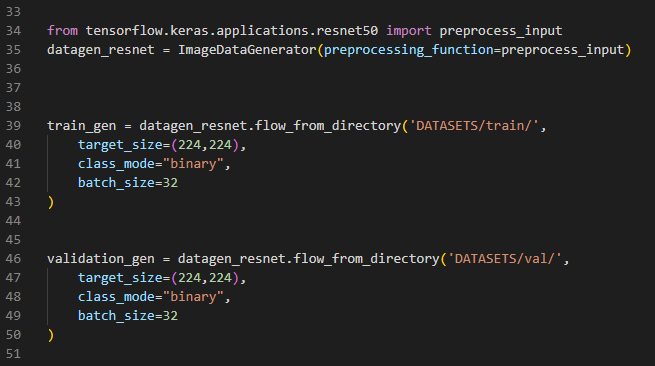
\includegraphics[width=0.6\textwidth]{figuras/normalization.png}
%  	\captionsetup{justification=centering}
% 	\vspace{-0.2cm}
%      \\\textbf{\footnotesize Fonte: \textit{GitHub}}
% 	\label{fig:normaliztion}
% \end{figure}

%%%%%%%%%%%%%%%%%%%%%%%     FUNÇÕES DE ATIVAÇÃO       %%%%%%%%%%%%%%%%%%%%%%

\subsubsection{\esp Camadas e Funções de Ativação do Modelo} \label{camadas}
Com as imagens de treinamento e validação pré-processadas, é necessário definir o modelo a ser utilizado. Foi feita a importação da rede neural \textit{ResNet} que aplica o método de \textit{Transfer Learning}. O modelo foi carregado na variável \textit{base\_model}, configurando parâmetros que indicam que a camada superior do modelo não será incluída (ou seja, foram usadas somente camadas convolucionais), e especificando o formato esperado das imagens de entrada para o modelo (já definidas anteriormente pelo método \textit{flow\_from\_directory}).

Um modelo ideal, na teoria, deve receber uma lista de camadas onde cada camada tem uma função específica. No diagrama da Figura \ref{fig:cnn} temos as camadas \textit{Conv\_1}, \textit{Conv\_2} e \textit{Max-Pooling}, responsáveis por extrair e detectar padrões das imagens, e a camada \textit{Fully-Connected}, que permite que o modelo aprenda padrões mais sofisticados. No modelo proposto, a \textit{ResNet} disponibiliza os dados extraídos, mas não implementa a camada \textit{Fully-Connected}.

\begin{figure}[ht]
 	\centering	
 	\caption[\hspace{0.1cm}Grade Computacional.]{Arquitetura completa de uma CNN que classifica dígitos manuscritos}
 	\vspace{-0.4cm}
 	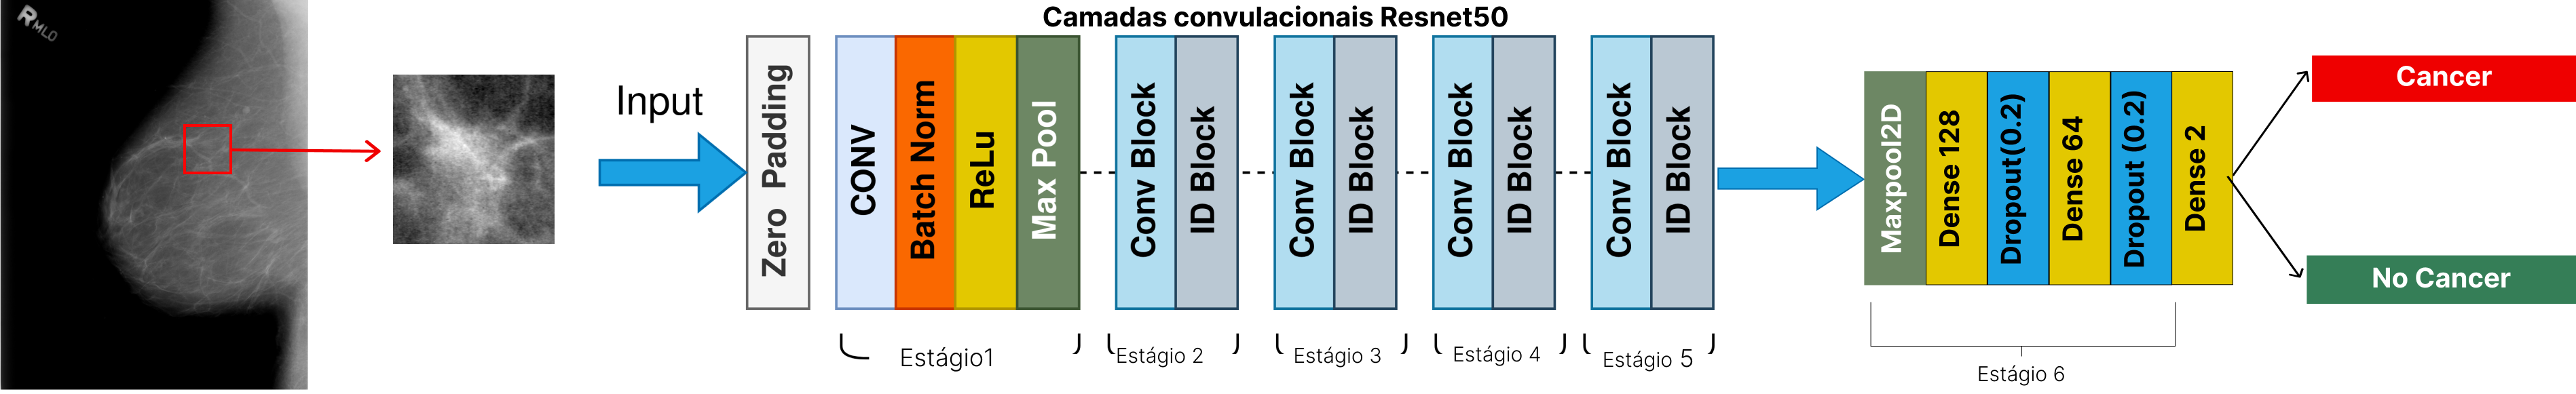
\includegraphics[width=0.9\textwidth]{figuras/cnn.png}
 	\captionsetup{justification=centering}
	\vspace{-0.2cm}
     \\\textbf{\footnotesize Fonte: \cite{towardsdatascienceimage}}
	\label{fig:cnn}
\end{figure}

A camada \textit{Max Pooling} reduz a dimensionalidade dos dados de entrada, agrupando \textit{pixels} de uma região para diminuir a variância a pequenas alterações, além de extrair características mais relevantes. Assim, essa camada reduz a resolução da imagem para dar uma maior especificidade em uma determinada característica, encurtando o conjunto de dados para o maior dado em um determinado conjunto selecionado.

Já a camada Convolucional opera aplicando um conjunto de filtros a uma imagem de entrada para extrair características importantes. A profundidade da saída de uma convolução é igual à quantidade de filtros aplicados. Quanto mais profundas são as camadas das convoluções, mais detalhados são os traços identificados com o Mapa de Ativação (do inglês \textit{Atactivation Map}). O filtro, também conhecido como \textit{Kernel}, é formado por pesos inicializados aleatoriamente, atualizando-os a cada nova entrada durante o processo de Retropropagação do Erro (do inglês \textit{Backpropagation}). A pequena região da entrada onde o filtro é aplicado é chamada de Campo Receptivo (do inglês \textit{Receptive Field}). Assim, é possível visualizar na Figura \ref{fig:conv2}, um filtro que representa a curva ao seu lado. Com essa combinação temos como resultado um número alto, indicando uma compatibilidade entre as curvas. Quando a imagem não possui nenhuma compatibilidade esse resultado chega mais próximo a zero.

\begin{figure}[ht]
 	\centering	
 	\caption[\hspace{0.1cm}Grade Computacional.]{Camada Convolucional}
 	\vspace{-0.4cm}
 	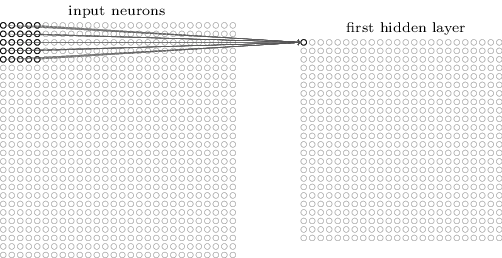
\includegraphics[width=1\textwidth]{figuras/conv.png}
 	\captionsetup{justification=centering}
	\vspace{-0.2cm}
     \\\textbf{\footnotesize Fonte: \cite{cnns}}
	\label{fig:conv2}
\end{figure}

Por fim, \textit{Flattern} é uma das camadas \textit{Fully Connected}, na qual sua entrada é a saída da camada anterior, e sua saída são N neurônios, sendo N a quantidade de classes do modelo para finalizar a classificação.


Para declarar o modelo da implementação, é necessário ter uma lista de camadas. É feita a importação de uma Interface de Programação de Aplicações (API, do inglês \textit{Application Programming Interface}) chamada \textit{Sequential}, que permite adicionar camadas sequencialmente ao modelo. Além disso, é importada também a camada \textit{Dense} que representa uma camada totalmente conectada, utilizada para mapear as entradas para as saídas. Juntamente com as camadas já citadas, temos a camada \textit{Flatten} usada para achatar os dados de entrada em um vetor unidimensional. Por fim, a camada \textit{GlobalAveragePooling2D} realiza a operação de \textit{pooling} médio, utilizada para reduzir a dimensionalidade dos recursos extraídos das camadas convolucionais anteriores. Para gerar arquivos de \textit{log} úteis para avaliar o desempenho do modelo, foi utilizado o \textit{TensorBoard}.

% \begin{figure}[ht]
%  	\centering	
%  	\caption[\hspace{0.1cm}Grade Computacional.]{Importação de Camadas}
%  	\vspace{-0.4cm}
%  	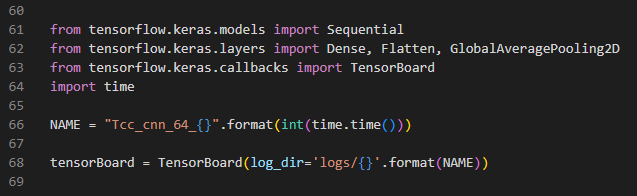
\includegraphics[width=0.5\textwidth]{figuras/layers.png}
%  	\captionsetup{justification=centering}
% 	\vspace{-0.2cm}
%      \\\textbf{\footnotesize Fonte: \textit{GitHub}}
% 	\label{fig:layers}
% \end{figure}


A variável \textit{base\_model}, já citada anteriormente, carrega as camadas convolucionais da rede neural \textit{ResNet}. Com isso, é necessário somente gerar as camadas \textit{Fully Connected}, que o \textit{ResNet} não consegue gerar. Para isso, a Figura x demonstra o código que percorre todas as camadas do modelo e define a propriedade \textit{trainable} como Falso para cada camada. Isso significa que as camadas do modelo base não foram treinadas durante o processo de treinamento subsequente. Ao definir a propriedade \textit{trainable}, as camadas do modelo base permaneceram com os pesos pré-treinados e não foram atualizadas durante o treinamento adicional. Após isso, foi definido o modelo de rede neural, passando uma lista de camadas. A camada \textit{base\_model} é a camada pré-treinada passada como entrada para o modelo. As outras camadas realizam operações para reduzir a dimensionalidade dos recursos extraídos de camadas anteriores.

% \begin{figure}[ht]
%  	\centering	
%  	\caption[\hspace{0.1cm}Grade Computacional.]{Modelo implementado com 10 épocas}
%  	\vspace{-0.4cm}
%  	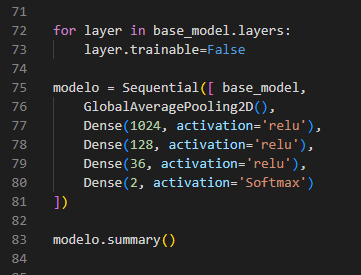
\includegraphics[width=0.6\textwidth]{figuras/model.png}
%  	\captionsetup{justification=centering}
% 	\vspace{-0.2cm}
%      \\\textbf{\footnotesize Fonte: \textit{GitHub}}
% 	\label{fig:model}
% \end{figure}

A camada \textit{Dense} realiza transformações lineares nos dados de entrada, e cada chamada contém parâmetros que se distinguem, assim como a quantidade de unidades (2, 36, 128 ou 1024) e a função do modo de ativação ('\textit{relu}', ou '\textit{softmax}'). A função de ativação \textit{Softmax}, representada na Figura \ref{fig:softmax}, é usada em redes neurais de classificação, forçando saída de uma rede neural a representar a probabilidade dos dados serem de uma das classes definidas. Sem ela, as saídas dos neurônios são simplesmente valores numéricos onde o maior indica a classe vencedora.
\begin{figure}[ht]
\centering
\begin{minipage}{0.45\textwidth}
  \centering
  \caption[\hspace{0.1cm}Grade Computacional.]{Função de Ativação \textit{softmax}}
  \vspace{-0.4cm}
  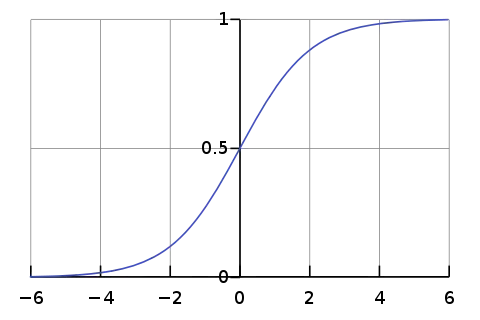
\includegraphics[width=\linewidth]{figuras/softmax.png}
  \captionsetup{justification=centering}
  \vspace{-0.2cm}
  \\\textbf{\footnotesize Fonte: \cite{softmax}}
  \label{fig:softmax}
\end{minipage}\hfill
\begin{minipage}{0.45\textwidth}
  \centering
  \caption[\hspace{0.1cm}Grade Computacional.]{Função de Ativação \textit{ReLU}}
  \vspace{-0.4cm}
  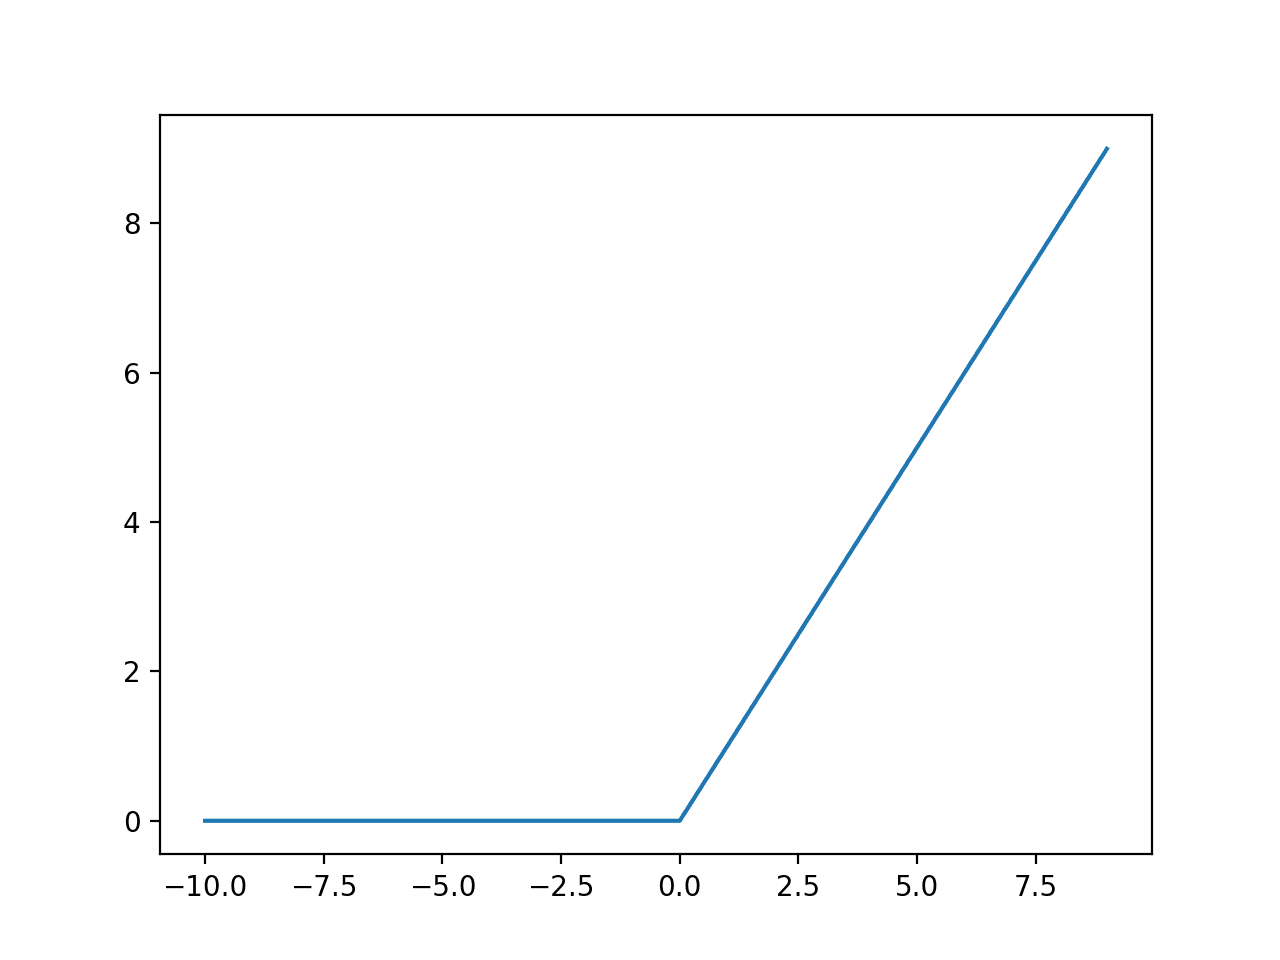
\includegraphics[width=\linewidth]{figuras/relu.png}
  \captionsetup{justification=centering}
  \vspace{-0.2cm}
  \\\textbf{\footnotesize Fonte: \cite{relu}}
  \label{fig:relu}
\end{minipage}
\end{figure}

Em contrapartida, a função de ativação Unidade Linear Retificada (ReLU, do inglês \textit{Rectified Linear Unit}), representada na Figura \ref{fig:relu}, pega os valores menores ou iguais à zero, e atribui como zero. É a função de ativação mais rápida para a geração de pesos e há somente suas classes.



%%%%%%%%%%%%%%%%%%%%%%%     TREINAMENTO       %%%%%%%%%%%%%%%%%%%%%%

\subsubsection{\esp Treinamento do Modelo} \label{treinamento}

A fim de treinar o modelo para identificar padrões e classificar as imagens, é necessário compilar o modelo com uma função de custo e otimizador, disponível na Figura training. A otimização de Adam é um método de decida de gradiente estocástico baseado na estimativa adaptativa de momentos de primeira e segunda ordem. De acordo com \citeonline{adam}, o método é computacionalmente eficiente, tem pouco requisito de memória, é invariante ao reescalonamento diagonal de gradientes e é adequado para problemas grandes em termos de dados. No modelo utilizado para a classificação do câncer, é definido o otimizador, juntamente com a taxa de aprendizado, que controla o tamanho dos passos dados pelo otimizador durante o treinamento. 

% \begin{figure}[ht]
%  	\centering	
%  	\caption[\hspace{0.1cm}Grade Computacional.]{Funções de custo e otimização}
%  	\vspace{-0.4cm}
%  	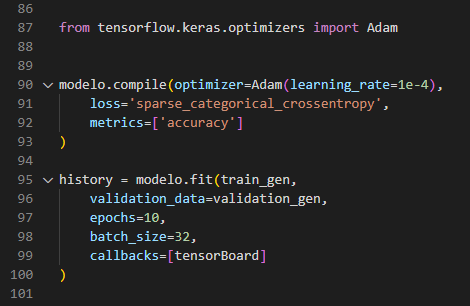
\includegraphics[width=0.5\textwidth]{figuras/training.png}
%  	\captionsetup{justification=centering}
% 	\vspace{-0.2cm}
%      \\\textbf{\footnotesize Fonte: \textit{GitHub}}
% 	\label{fig:training}
% \end{figure}

Nesse caso, a taxa é definida como \ensuremath{1 \times 10^{-4}}. Além disso, é especificada a função de perda utilizada para treinar o modelo (\textit{sparse\_categorical\_crossentropy}), onde há dois ou mais rótulos de saída e calcula a diferença entre as probabilidades preditas pelo modelo e as classes reais dos dados de treinamento. Por fim, é especificada a métrica utilizada para avaliar o desempenho do modelo durante o treinamento. A métrica escolhida foi a acurácia, que mede a proporção de exemplos classificados corretamente em relação ao total de exemplos. 

Após compilar o modelo, ele é de fato treinado utilizando os dados de treinamento e validação, atribuindo o histórico de treinamento que contém métricas de perda e avaliação, na variável \textit{history}. O método \textit{fit} treina o modelo utilizando os dados fornecidos, passando alguns parâmetros como configuração. A variável \textit{train\_gen}, mencionada na seção \ref{transfer}, representa o gerador de dados de treinamento, em conjunto à \textit{validation\_gen} que representa o gerador de dados de validação. Em seguida são definidos parâmetros como a quantidade de épocas (passagem completa pelos dados de treinamento), tamanho do lote (número de exemplos de treinamento usados em cada atualização do modelo), e uma lista opcional de objetos de Retornos de Chamada (do inglês \textit{Callback}), que executam ações específicas em momentos específicos durante o treinamento. No modelo proposto, somente um único \textit{Callback} chamado \textit{tensorBoard} está sendo passado. Além disso, o tamanho do lote é fixo em 32, e a quantidade de épocas foi definida em dois valores, para dois modelos diferentes à serem validados. O primeiro modelo utiliza de 10 épocas, e o segundo modelo utiliza de 7 épocas.


%%%%%%%%%%%%%%%%%%%%%%%%%%%%%%%%%%%%%%%%%%%%%%%%%%%%%%%%%%%%%%%%%%%%%%%%%
%%%%%%%%%%%%%%%%%%%%%%%%%      RESULTADOS      %%%%%%%%%%%%%%%%%%%%%%%%%%
%%%%%%%%%%%%%%%%%%%%%%%%%%%%%%%%%%%%%%%%%%%%%%%%%%%%%%%%%%%%%%%%%%%%%%%%%

\section{\esp Experimentos e Resultados} \label{results}


%%%%%%%%%%%%%%%%%%%%%%%     PRELIMINARES       %%%%%%%%%%%%%%%%%%%%%%

\subsection{\esp Resultados Preliminares} \label{prelim}

Para avaliar os resultados dos modelos propostos, utilizamos a biblioteca \textit{Pandas} que manipula e faz a análise de dados. Outrossim, é feita a análise da acurácia e perda do modelo, onde o histórico do treino pode ser observado na Tabela \ref{tab:history7}.

% \begin{table}[h]
%   \centering
%   \caption{Histórico de treino com 10 épocas}
%    \label{tab:history10}
% \begin{tabular}{|c|c|c|c|c|} 
%   \hline
%    epochs & loss & accuracy & val\_loss & val\_accuracy \\
%   \hline
%     0 & 0.268681 & 0.891832 & 0.143105 & 0.943488 \\
%     1 & 0.127448 & 0.953642 & 0.082275 & 0.974614 \\
%     2 & 0.083150 & 0.972185 & 0.065914 & 0.980795 \\
%     3 & 0.062938 & 0.979249 & 0.044413 & 0.986976 \\
%     4 & 0.050511 & 0.982119 & 0.030504 & 0.991832 \\
%     5 & 0.035133 & 0.990287 & 0.038080 & 0.989404 \\
%     6 & 0.024261 & 0.994040 & 0.016370 & 0.998455 \\
%     7 & 0.017749 & 0.995806 & 0.010396 & 0.999559 \\
%     8 & 0.021589 & 0.992715 & 0.050530 & 0.976821 \\
%     9 & 0.013694 & 0.997351 & 0.005069 & 1.000000 \\
%   \hline
% \end{tabular}

% \end{table}

\begin{table}[h]
  \centering
  \caption{Histórico de treino com 7 épocas}
   \label{tab:history7}
\begin{tabular}{|c|c|c|c|c|} 
  \hline
   epochs & loss & accuracy & val\_loss & val\_accuracy \\
  \hline
0 & 0.289751 & 0.887196 & 0.172350 & 0.952539 \\
1 & 0.148235 & 0.945475 & 0.108529 & 0.973289 \\
2 & 0.098310 & 0.964680 & 0.080067 & 0.969536 \\
3 & 0.064811 & 0.979249 & 0.043451 & 0.986093 \\
4 & 0.045955 & 0.986313 & 0.031383 & 0.993378 \\
5 & 0.035269 & 0.987417 & 0.021023 & 0.996909 \\
6 & 0.025187 & 0.992274 & 0.014035 & 0.997572 \\
  \hline
\end{tabular}

\end{table}

Além disso, as Figuras \ref{fig:acc7} e \ref{fig:loss7}, representam gráficos de acurácia e perda com 7 épocas, quantidade definida a partir de testes empíricos. O modelo se comporta da maneira esperada, e sem sinais de Sobreajuste (do inglês \textit{Overfitting}), comportamento indesejável de \textit{Machine Learning} que ocorre quando o modelo fornece previsões precisas para dados de treinamento, mas não para novos dados. 
% Em contrapartida, na Figura \ref{fig:loss10}, o erro diminui à medida que o número de épocas aumentam. No entanto, é importante ressaltar que ocorre novamente o fenômeno de \textit{Overfitting} na época 8, onde o modelo começa a se ajustar excessivamente, levando a uma perda de generalização. 

% \begin{figure}[ht]
%  	\centering	
%  	\caption[\hspace{0.1cm}Grade Computacional.]{Gráfico de acurácia com 10 épocas}
%  	\vspace{-0.4cm}
%  	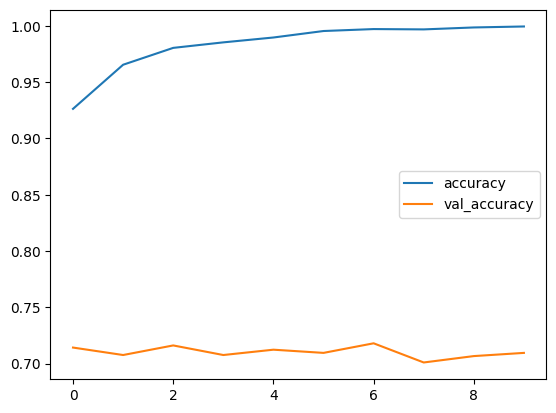
\includegraphics[width=0.5\textwidth]{figuras/accuracy_10.png}
%  	\captionsetup{justification=centering}
% 	\vspace{-0.2cm}
%      \\\textbf{\footnotesize Fonte: \textit{GitHub}}
% 	\label{fig:acc10}
% \end{figure}

% \begin{figure}[ht]
%  	\centering	
%  	\caption[\hspace{0.1cm}Grade Computacional.]{Gráfico de perda com 10 épocas}
%  	\vspace{-0.4cm}
%  	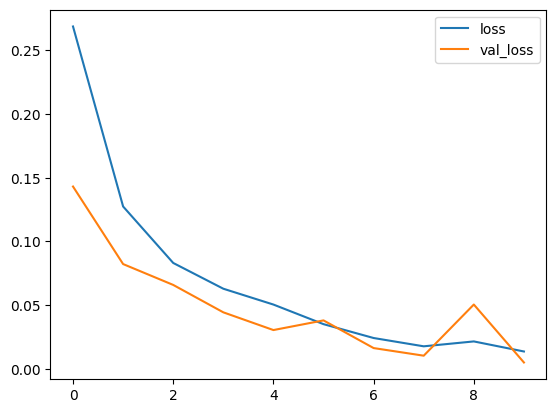
\includegraphics[width=0.5\textwidth]{figuras/loss_10.png}
%  	\captionsetup{justification=centering}
% 	\vspace{-0.2cm}
%      \\\textbf{\footnotesize Fonte: \textit{GitHub}}
% 	\label{fig:loss10}
% \end{figure}


% Por esses motivos, um modelo com somente 8 épocas foi treinado. O histórico do treino pode ser observado na Tabela \ref{tab:history7}. As Figuras \ref{fig:acc7} e \ref{fig:loss7} representam, respectivamente, os gráficos de acurácia e perda com 7 épocas. Após feita a alteração é possível ver que o modelo se comporta claramente de uma maneira melhor e da maneira esperada (sem \textit{Overfitting}).

% \begin{figure}[ht]
%  	\centering	
%  	\caption[\hspace{0.1cm}Grade Computacional.]{Modelo implementado com 7 épocas}
%  	\vspace{-0.4cm}
%  	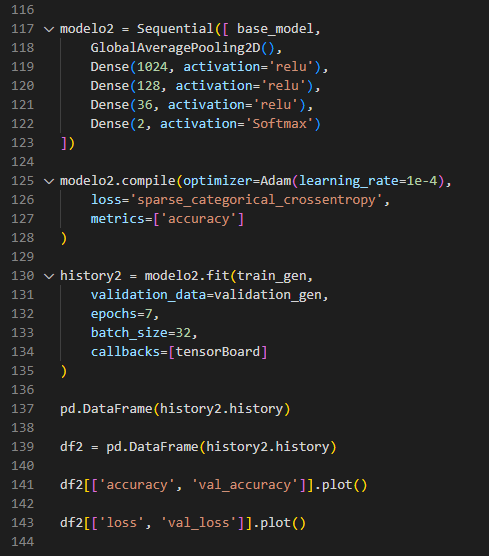
\includegraphics[width=0.5\textwidth]{figuras/model_7.png}
%  	\captionsetup{justification=centering}
% 	\vspace{-0.2cm}
%      \\\textbf{\footnotesize Fonte: \textit{GitHub}}
% 	\label{fig:model7}
% \end{figure}

\begin{figure}[ht]
\centering
\begin{minipage}{0.45\textwidth}
  \centering
  \caption[\hspace{0.1cm}Grade Computacional.]{Gráfico de acurácia com 7 épocas}
  \vspace{-0.4cm}
  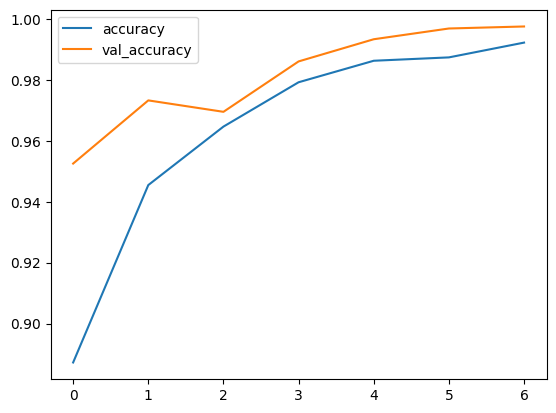
\includegraphics[width=\linewidth]{figuras/accuracy_7.png}
  \captionsetup{justification=centering}
  \vspace{-0.2cm}
  \\\textbf{\footnotesize Fonte: \textit{GitHub}}
  \label{fig:acc7}
\end{minipage}\hfill
\begin{minipage}{0.45\textwidth}
  \centering
  \caption[\hspace{0.1cm}Grade Computacional.]{Gráfico de perda com 7 épocas}
  \vspace{-0.4cm}
  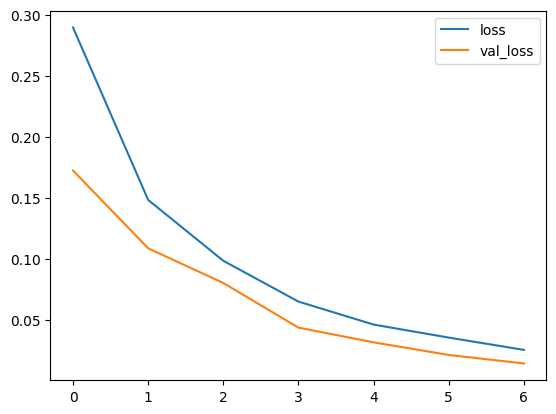
\includegraphics[width=\linewidth]{figuras/loss_7.png}
  \captionsetup{justification=centering}
  \vspace{-0.2cm}
  \\\textbf{\footnotesize Fonte: \textit{GitHub}}
  \label{fig:loss7}
\end{minipage}
\end{figure}



%%%%%%%%%%%%%%%%%%%%%%%     PREDIÇÕES       %%%%%%%%%%%%%%%%%%%%%%

\subsection{\esp Predições} \label{pred}

Por fim, importamos a biblioteca \textit{nunpy} e definimos a função de predição que irá classificar uma imagem como sendo um paciente com câncer ou sem câncer. Essa função, ilustrada na Figura \ref{fig:predicao}, recebe como entrada um modelo de \textit{Machine Learning} e o caminho de um arquivo de imagem, e retorna o resultado da classificação. Para isso, a função \textit{predicao} armazena a imagem em uma variável, redimensionando-a para o tamanho que a rede neural requisita (224x224 \textit{pixels}). Após isso, a função de predição converte a imagem em um vetor, realizando o pré-processamento com a função  \textit{preprocess\_input}, especificada na seção \ref{transfer}. Além disso, reordena o vetor da imagem para ter uma amostra com as dimensões já especificadas, definindo o número de canais de cor para 3. A função de predição então realiza a previsão do modelo guardando o resultado numa variável que contém as probabilidades associadas a cada classe, e encontra o índice da classe com a maior probabilidade. Finalmente, cria um dicionário que mapeia os índices das classes para seus rótulos correspondentes com base nos índices definidos pelo gerador de imagens de treinamento, exibindo a imagem com a predição.



\begin{figure}[ht]
 	\centering	
 	\caption[\hspace{0.1cm}Grade Computacional.]{Definição da função de predição}
 	\vspace{-0.4cm}
 	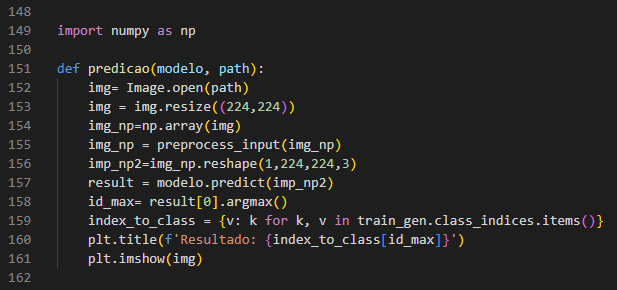
\includegraphics[width=0.5\textwidth]{figuras/predicao.png}
 	\captionsetup{justification=centering}
	\vspace{-0.2cm}
     \\\textbf{\footnotesize Fonte: \textit{GitHub}}
	\label{fig:predicao}
\end{figure}

% Ainda na Figura \ref{fig:predicao}, temos as chamadas dos métodos para retornar a predição. É possível observar que na Figura \ref{fig:predicao1}, é passada uma imagem de validação para o modelo com 10 épocas de um paciente com câncer. O resultado do modelo retornou uma classificação correta, apontando que a imagem é de um paciente sem câncer. Já na Figura \ref{fig:predicao2}, é passada uma imagem de validação, ainda com o modelo de 10 épocas, de um paciente sem câncer. Novamente, o modelo retorna o resultado correto.

% \begin{figure}[ht]
%  	\centering	
%  	\caption[\hspace{0.1cm}Grade Computacional.]{Predição de paciente com câncer com 10 épocas}
%  	\vspace{-0.4cm}
%  	\includegraphics[width=0.5\textwidth]{figuras/model10pred1.png}
%  	\captionsetup{justification=centering}
% 	\vspace{-0.2cm}
%      \\\textbf{\footnotesize Fonte: \textit{GitHub}}
% 	\label{fig:predicao1}
% \end{figure}

% \begin{figure}[ht]
%  	\centering	
%  	\caption[\hspace{0.1cm}Grade Computacional.]{Predição de paciente sem câncer com 10 épocas}
%  	\vspace{-0.4cm}
%  	\includegraphics[width=0.5\textwidth]{figuras/model10pred2.png}
%  	\captionsetup{justification=centering}
% 	\vspace{-0.2cm}
%      \\\textbf{\footnotesize Fonte: \textit{GitHub}}
% 	\label{fig:predicao2}
% \end{figure}


É possível observar que na Figura \ref{fig:predicao3}, é passada uma imagem de validação para o modelo de um paciente com câncer. O resultado do modelo retornou uma classificação correta, apontando que a imagem é de um paciente sem câncer. Já na Figura \ref{fig:predicao4}, é passada uma imagem de validação de um paciente sem câncer. Novamente, o modelo retorna o resultado correto.

% Utilizando o modelo com 7 épocas, o resultado ainda é satisfatório. Na Figura \ref{fig:predicao3} temos que a chamada é de um paciente sem câncer, e o modelo retorna o resultado correto. O mesmo comportamento acontece ao passar uma imagem de um paciente sem câncer, Figura \ref{fig:predicao4}, onde o modelo também retorna que o paciente não tem câncer.

\begin{figure}[ht]
\centering
\begin{minipage}{0.45\textwidth}
  \centering
  \caption[\hspace{0.1cm}Grade Computacional.]{Predição de paciente com câncer}
  \vspace{-0.4cm}
  \includegraphics[width=\linewidth]{figuras/model7pred1.png}
  \captionsetup{justification=centering}
  \vspace{-0.2cm}
  \\\textbf{\footnotesize Fonte: \textit{GitHub}}
  \label{fig:predicao3}
\end{minipage}\hfill
\begin{minipage}{0.45\textwidth}
  \centering
  \caption[\hspace{0.1cm}Grade Computacional.]{Predição de paciente sem câncer}
  \vspace{-0.4cm}
  \includegraphics[width=\linewidth]{figuras/model7pred2.png}
  \captionsetup{justification=centering}
  \vspace{-0.2cm}
  \\\textbf{\footnotesize Fonte: \textit{GitHub}}
  \label{fig:predicao4}
\end{minipage}
\end{figure}



% \subsection{\esp Cronograma} \label{cronograma}
% Descomentar tabela ou colocar imagem

% 1. revisao dos resultados e feedback
% 2. trocar base de dados para uma com mais imagens e as imagens sendo termograficas
% 3. melhorar o modelo e resultados
% 4. implementar interface gráfica
% \begin{table}[htbp]
%     \centering
%     \caption{Cronograma}
%     \label{tab:exemplo}
%     \begin{tabular}{|c|c|c|c|c|c|c|}
%         \hline
%         \textbf{} & \textbf{Tarefa} & \textbf{Julho} & \textbf{Agosto} & \textbf{Setembro} & \textbf{Outubro} & \textbf{Novembro}\\
%         \hline
%         1 & Revisão de resultados & x & x & x & x & x  \\
%         \hline
%         2 & Trocar a base de dados  & x & x & x & x & x  \\
%         \hline
%         3 & Melhorar acurácia dos resultados  & x & x & x & x &  x\\
%         \hline
%         4 & Implementar interface gráfica  & x & x & x & x & x \\
%         \hline
%         5 & Tarefa 5  & x & x & x & x & x  \\
%         \hline
%         6 & Tarefa 6  & x & x & x & x & x  \\
%         \hline
%         7 & Tarefa 7  & x & x & x & x & x  \\
%         \hline
%         8 & Tarefa 8  & x & x & x & x & x  \\
%         \hline
%     \end{tabular}
% \end{table}